\chapter{Oxydation et réduction des alcènes}\label{ch:b2:alkene-redox}

Une colle époxy bicomposant se présente en deux tubes~: l'un contient des molécules terminées
par des cycles \omterm{def:b2:alkene-redox:epoxide}{époxyde}, cycles à trois atomes formés de deux carbones et d'un oxygène~; l'autre
une amine. Après mélange, les cycles tendus s'ouvrent les uns après les autres et la pâte durcit
en un réseau rigide. Les alcènes sont la matière première de ces cycles, d'alcools placés là où
la règle de Markovnikov ne les mettrait jamais, de diols de géométrie choisie, et des petits
fragments qui indiquaient autrefois aux chimistes la position d'une double liaison dans une
molécule. Ce chapitre ajoute aux additions électrophiles du volume de première année les
réactions qui réduisent ou oxydent la double liaison, et la stéréochimie que chacune impose.

\begin{recall}
Le volume de première année~: additions électrophiles, règle de Markovnikov, ions halogénonium,
additions syn et anti, hydratation des alcènes, nombres d'oxydation du carbone, donneurs
d'hydrure, chimiosélectivité, composés méso et mélanges racémiques, réactions stéréospécifiques.
\Cref{ch:b2:catalytic-cycles}~: le cycle d'hydrogénation du catalyseur de
Wilkinson.
\end{recall}

\begin{omfigure}
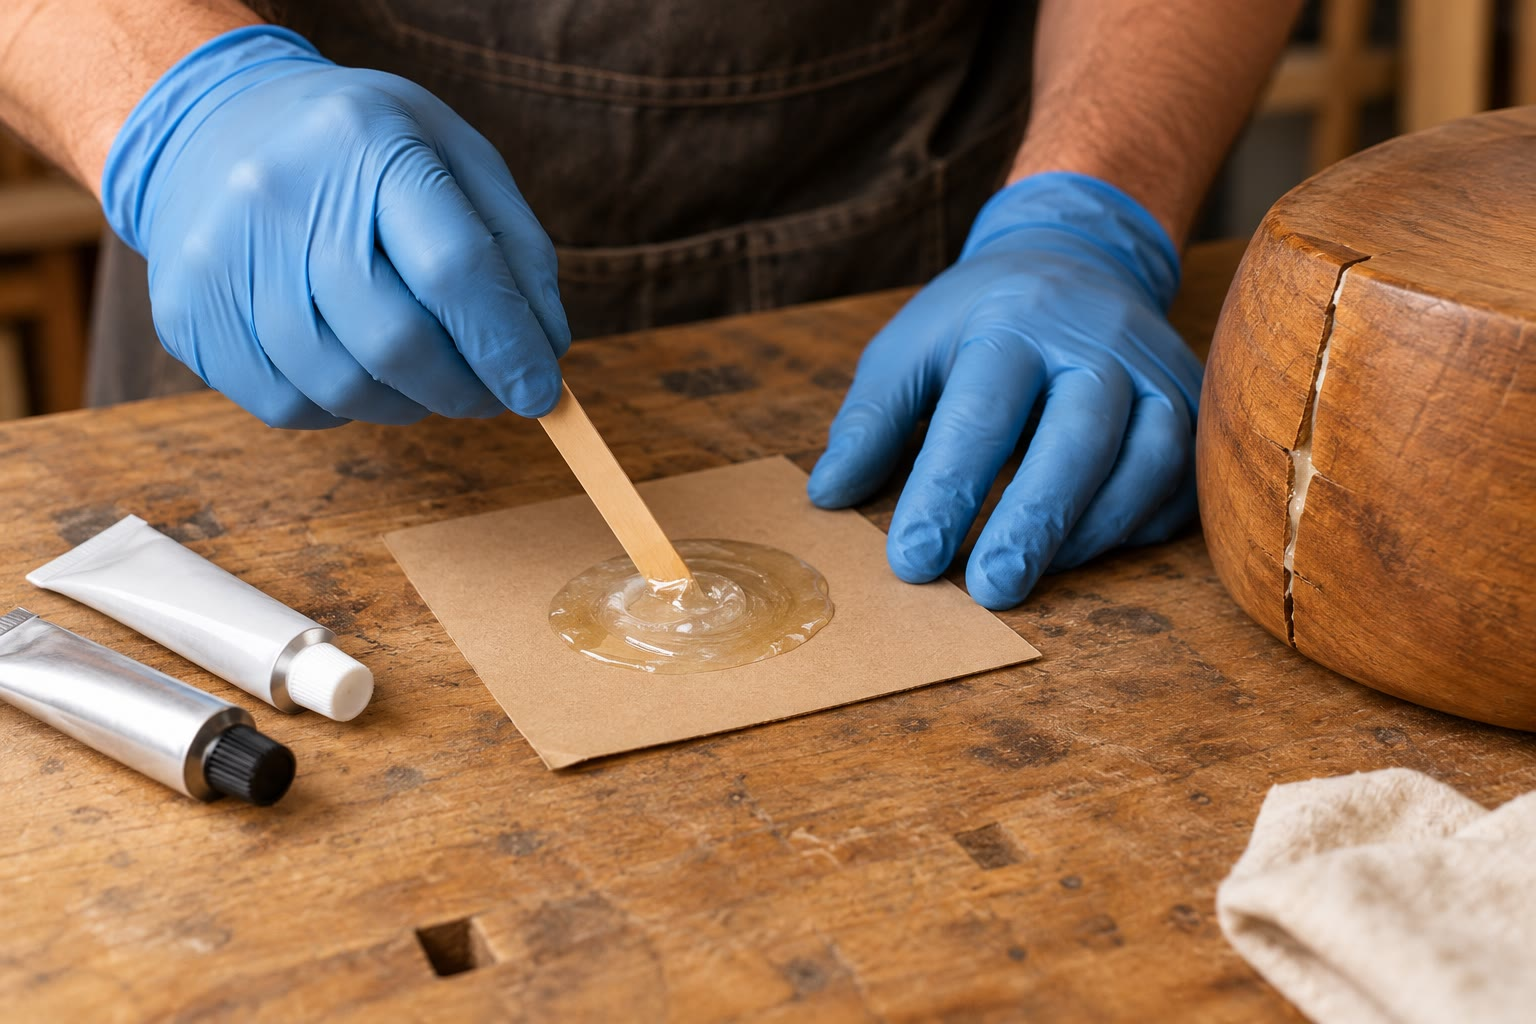
\includegraphics[width=0.6\linewidth]{images/book3/ai/b2-21-epoxy.jpg}

{\small Mélange d'une colle époxy bicomposant~: la résine, porteuse de groupes \omterm{def:b2:alkene-redox:epoxide}{époxyde}, et le
durcisseur, une amine, réagissent dès qu'ils se rencontrent~; les cycles s'ouvrent et relient les
molécules en un réseau solide.}
\end{omfigure}

\section{Hydrogénation catalytique}

\begin{definition}[Hydrogénation catalytique]\label{def:b2:alkene-redox:hydrogenation}
Une \emph{hydrogénation catalytique}\index{hydrogenation catalytique@hydrogénation catalytique} additionne le dihydrogène sur une
liaison multiple en présence d'un catalyseur~: un métal finement divisé (palladium sur
charbon, platine, nickel) en catalyse hétérogène, ou un complexe soluble comme celui
de Wilkinson en catalyse homogène.
\end{definition}

Sur une surface métallique, le dihydrogène et l'alcène sont tous deux retenus, la liaison \ce{H-H}
est rompue en atomes d'hydrogène de surface, et ceux-ci sont transférés l'un après l'autre aux
atomes de carbone de l'alcène, couché à plat sur le métal.

\begin{proposition}[Addition syn]\label{prop:b2:alkene-redox:syn-hydrogenation}
L'\omterm{def:b2:alkene-redox:hydrogenation}{hydrogénation catalytique} apporte les deux atomes d'hydrogène sur la même face de la double
liaison. Un alcyne hydrogéné sur un catalyseur au palladium empoisonné s'arrête à l'alcène, qui
est l'isomère (\textit{Z}).
\end{proposition}

\begin{proof}[Argument]
L'alcène est lié au catalyseur par une de ses faces, et les deux hydrogènes viennent du
catalyseur, donc de cette face~: addition syn. Avec un alcyne, les deux hydrogènes ajoutés sur la
triple liaison sont du même côté, en cis l'un par rapport à l'autre~: l'alcène (\textit{Z}). Un
catalyseur partiellement désactivé (palladium sur carbonate de calcium avec un sel de plomb et de
la quinoléine) fixe l'alcyne bien plus fortement que l'alcène formé, qui quitte la surface
avant une seconde addition.
\end{proof}

\section{Hydroboration--oxydation}

\begin{definition}[Hydroboration]\label{def:b2:alkene-redox:hydroboration}
Une \emph{hydroboration}\index{hydroboration} additionne une liaison B--H d'un borane sur une
liaison \ce{C=C}~; suivie d'une oxydation par le peroxyde d'hydrogène en milieu basique, elle
transforme l'alcène en un alcool dont le groupe hydroxyle se trouve sur le carbone le moins
substitué~: une \emph{orientation anti-Markovnikov}\index{orientation anti-Markovnikov}.
\end{definition}

\begin{omfigure}
\setchemfig{atom sep=1.8em}
\schemestart[][west]
\chemfig{H_3C-[:30]CH=[:-30]CH_2}
\+ \chemfig{H-BH_2}
\arrow{->[addition syn]}
\chemfig{H_3C-[:30]CH_2-[:-30]CH_2-[:30]BH_2}
\arrow{->[\ce{H2O2}][\ce{HO-}]}
\chemfig{H_3C-[:30]CH_2-[:-30]CH_2-[:30]OH}
\schemestop
\par\vspace{6pt}

{\small Hydroboration--oxydation du propène. Le borane s'additionne en une seule étape, le bore
sur le carbone terminal et l'hydrogène sur le carbone interne, tous deux sur la même face~;
l'oxydation remplace le bore par \ce{OH} avec rétention de configuration. Il se forme du
propan-1-ol, et non le propan-2-ol de l'hydratation en milieu acide.}
\end{omfigure}

\begin{proposition}[Orientation de l'hydroboration]\label{prop:b2:alkene-redox:hydroboration-regio}
Le bore se fixe sur le carbone le moins substitué de la double liaison, et l'hydrogène sur le
plus substitué~; l'addition est syn.
\end{proposition}

\begin{proof}[Argument]
Le bore, qui possède une orbitale p vide, est l'électrophile~: dans l'état de transition à quatre
centres (les deux carbones, le bore et l'hydrogène), la liaison au bore se forme un peu avant la
liaison C--H, et une charge partielle positive apparaît sur l'autre carbone, mieux portée par le
plus substitué~; le groupe boré, encombrant, préfère aussi l'extrémité la moins encombrée. Les
deux nouvelles liaisons se forment sur une même face, en une étape concertée~: syn.
\end{proof}

\begin{proposition}[Oxydation avec rétention]\label{prop:b2:alkene-redox:retention}
L'oxydation d'un alkylborane par le peroxyde d'hydrogène en milieu basique remplace chaque
liaison C--B par une liaison C--OH avec rétention de configuration du carbone.
\end{proposition}

\begin{proof}[Argument]
L'anion hydroperoxyde s'additionne sur le bore~; un groupe alkyle migre ensuite du bore vers
l'oxygène voisin, avec son doublet d'électrons, tandis que l'hydroxyde part~; le carbone garde
ses liaisons du même côté tout au long. L'hydrolyse de la liaison B--O libère l'alcool.
\end{proof}

\section{Époxydes}

\begin{definition}[Époxyde]\label{def:b2:alkene-redox:epoxide}
Un \emph{époxyde}\index{epoxyde@époxyde} (oxirane) est un éther cyclique dont le cycle à trois atomes
comporte deux carbones et un oxygène. Une \emph{époxydation}\index{epoxydation@époxydation} transforme
un alcène en époxyde, le plus souvent au moyen d'un \emph{peroxyacide}\index{peroxyacide} \ce{RCO3H}, qui
transfère un atome d'oxygène à la double liaison.
\end{definition}

\begin{omfigure}
\setchemfig{atom sep=2em}
\schemestart
\chemfig{R-[:30]CH=[:-30]CH-[:30]R}
\+ \chemfig{Ar-C(=[2]O)-O-O-H}
\arrow{->}
\chemfig{[:-60]CH(-[:210]R)*3(-CH(-[:-30]R)-O-)}
\+ \chemfig{Ar-C(=[2]O)-OH}
\schemestop
\par\vspace{6pt}

{\small \omterm{def:b2:alkene-redox:epoxide}{Époxydation} par un \omterm{def:b2:alkene-redox:epoxide}{peroxyacide} (Ar~: par exemple un groupe 3-chlorophényle). L'oxygène
terminal du \omterm{def:b2:alkene-redox:epoxide}{peroxyacide} est transféré à la double liaison en une seule étape, les deux liaisons
C--O se formant sur la même face.}
\end{omfigure}

\begin{proposition}[Époxydation stéréospécifique]\label{prop:b2:alkene-redox:epoxidation}
L'\omterm{def:b2:alkene-redox:epoxide}{époxydation} par un \omterm{def:b2:alkene-redox:epoxide}{peroxyacide} est stéréospécifique~: un alcène (\textit{Z}) donne l'\omterm{def:b2:alkene-redox:epoxide}{époxyde}
cis, un alcène (\textit{E}) l'\omterm{def:b2:alkene-redox:epoxide}{époxyde} trans.
\end{proposition}

\begin{proof}
L'oxygène est transféré en une seule étape concertée sur une face de la double liaison, qui ne
tourne pas entre-temps~: les positions relatives des substituants sont conservées.
\end{proof}

\begin{proposition}[Ouverture des époxydes]\label{prop:b2:alkene-redox:opening}
Un nucléophile ouvre un \omterm{def:b2:alkene-redox:epoxide}{époxyde} en attaquant un carbone par la face opposée à l'oxygène
(ouverture anti, avec inversion de ce carbone). En milieu basique, il attaque le carbone le moins
encombré~; en milieu acide, le plus substitué.
\end{proposition}

\begin{proof}[Argument]
La tension du cycle rend les liaisons C--O faciles à rompre. Avec un nucléophile fort et sans
acide, l'ouverture est une substitution bimoléculaire, et le carbone le moins encombré est le
plus facile à atteindre. En milieu acide, l'oxygène est protoné~; la liaison C--O vers le carbone
le plus substitué s'allonge le plus, ce carbone portant la plus grande charge partielle positive,
et même un nucléophile faible (l'eau, un alcool) attaque là --- toujours par l'arrière, donc
toujours en anti.
\end{proof}

\begin{omfigure}
\setchemfig{atom sep=2em}
\schemestart
\chemfig{[:-60]C(-[:210]H_3C)(-[:150]H_3C)*3(-CH_2-O-)}
\arrow{->[\ce{CH3O-}][\ce{CH3OH}]}[,1.4]
\chemfig{H_3C-C(-[2]CH_3)(-[6]OH)-CH_2-OCH_3}
\schemestop

\medskip
\schemestart
\chemfig{[:-60]C(-[:210]H_3C)(-[:150]H_3C)*3(-CH_2-O-)}
\arrow{->[\ce{CH3OH}][\ce{H+}]}[,1.4]
\chemfig{H_3C-C(-[2]CH_3)(-[6]OCH_3)-CH_2-OH}
\schemestop
\par\vspace{6pt}

{\small Ouverture du 2,2-diméthyloxirane par le méthanol. En haut, avec le méthanolate~: attaque
sur le \ce{CH2}, le carbone le moins encombré. En bas, en milieu acide~: attaque sur le carbone le
plus substitué, qui porte l'essentiel de la charge positive de l'\omterm{def:b2:alkene-redox:epoxide}{époxyde} protoné.}
\end{omfigure}

\section{Dihydroxylation}

\begin{definition}[Dihydroxylation]\label{def:b2:alkene-redox:dihydroxylation}
Une \emph{dihydroxylation}\index{dihydroxylation} transforme un alcène en un diol-1,2 en ajoutant
un groupe \ce{OH} sur chaque carbone de la double liaison.
\end{definition}

Le tétraoxyde d'osmium, en quantité catalytique avec un réoxydant, et le permanganate dilué à
froid apportent les deux oxygènes par l'intermédiaire d'un ester cyclique, sur une même face~:
une \omterm{def:b2:alkene-redox:dihydroxylation}{dihydroxylation} syn. Une \omterm{def:b2:alkene-redox:epoxide}{époxydation} suivie d'une ouverture par l'eau en milieu acide donne
le diol anti.

\begin{proposition}[Diols syn et anti]\label{prop:b2:alkene-redox:diols}
À partir du (\textit{Z})-but-2-ène, la \omterm{def:b2:alkene-redox:dihydroxylation}{dihydroxylation} syn donne le méso-butane-2,3-diol et la
voie de l'\omterm{def:b2:alkene-redox:epoxide}{époxyde} donne le mélange racémique des diols (2\textit{R},3\textit{R}) et
(2\textit{S},3\textit{S})~; à partir du (\textit{E})-but-2-ène, les résultats sont échangés.
\end{proposition}

\begin{proof}
Dans le (\textit{Z})-but-2-ène, les deux méthyles sont du même côté. Ajouter deux \ce{OH} sur une
même face donne un diol dans lequel, écrit dans la conformation éclipsée de l'ancienne double
liaison, les deux \ce{OH} sont d'un côté et les deux méthyles de l'autre~: un plan miroir passe
entre C2 et C3, c'est le composé méso. La voie de l'\omterm{def:b2:alkene-redox:epoxide}{époxyde} place les deux \ce{OH} sur des faces
opposées (anti)~: le plan miroir disparaît, et l'attaque sur l'un ou l'autre carbone de l'\omterm{def:b2:alkene-redox:epoxide}{époxyde}
achiral, également probable, donne les deux énantiomères en quantités égales. Pour l'alcène
(\textit{E}), chaque étape inverse la relation entre les méthyles, ce qui échange les résultats.
\end{proof}

\begin{omfigure}
\begin{tikzpicture}[font=\small]
  \begin{scope}
    \draw[thick] (0,0) -- (0,1.2);
    \draw[thick] (0,1.2) -- (-0.7,1.45); \draw[thick] (0,1.2) -- (0.7,1.45);
    \node[anchor=east] at (-0.7,1.45) {\ce{HO}}; \node[anchor=west] at (0.7,1.45) {\ce{CH3}};
    \draw[thick] (0,0) -- (-0.7,0.25); \draw[thick] (0,0) -- (0.7,0.25);
    \node[anchor=east] at (-0.7,0.25) {\ce{HO}}; \node[anchor=west] at (0.7,0.25) {\ce{CH3}};
    \node[anchor=south] at (0,1.25) {\scriptsize H};
    \node[anchor=north] at (0,-0.05) {\scriptsize H};
    \draw[densely dashed, omThm] (-1.6,0.6) -- (1.6,0.6);
    \node at (0,-1.0) {syn~: méso};
  \end{scope}
  \begin{scope}[xshift=6.5cm]
    \draw[thick] (0,0) -- (0,1.2);
    \draw[thick] (0,1.2) -- (-0.7,1.45); \draw[thick] (0,1.2) -- (0.7,1.45);
    \node[anchor=east] at (-0.7,1.45) {\ce{HO}}; \node[anchor=west] at (0.7,1.45) {\ce{CH3}};
    \draw[thick] (0,0) -- (-0.7,0.25); \draw[thick] (0,0) -- (0.7,0.25);
    \node[anchor=east] at (-0.7,0.25) {\ce{H3C}}; \node[anchor=west] at (0.7,0.25) {\ce{OH}};
    \node[anchor=south] at (0,1.25) {\scriptsize H};
    \node[anchor=north] at (0,-0.05) {\scriptsize H};
    \node[align=center] at (0,-1.1) {anti~: un énantiomère\\ (formé avec son image dans un miroir)};
  \end{scope}
\end{tikzpicture}

{\small Les deux butane-2,3-diols issus du (\textit{Z})-but-2-ène, schématiques (liaison C2--C3
verticale, les deux groupes de chaque carbone dessinés à gauche et à droite). L'addition syn
place les deux \ce{OH} du même côté~: un plan miroir interne (en tirets), le composé méso.
L'addition anti les place de part et d'autre~: un diol chiral, formé avec son énantiomère.}
\end{omfigure}

\section{Coupure oxydante}

\begin{definition}[Coupure oxydante]\label{def:b2:alkene-redox:cleavage}
Une \emph{coupure oxydante}\index{coupure oxydante} rompt les deux liaisons d'une double liaison
\ce{C=C} et transforme chaque carbone en groupe carbonyle ou carboxyle. Dans une
\emph{ozonolyse}\index{ozonolyse}, l'alcène réagit avec l'ozone et l'ozonide intermédiaire
est décomposé lors d'une seconde étape, le traitement.
\end{definition}

\begin{proposition}[Produits de l'ozonolyse]\label{prop:b2:alkene-redox:ozonolysis}
L'\omterm{def:b2:alkene-redox:cleavage}{ozonolyse} scinde chaque liaison \ce{C=C} en deux groupes \ce{C=O}. Avec un traitement
réducteur (zinc et acide, ou sulfure de diméthyle), un carbone porteur d'un hydrogène donne un
aldéhyde~; avec un traitement oxydant (peroxyde d'hydrogène), il donne un acide carboxylique.
Un carbone porteur de deux groupes carbonés donne une cétone dans les deux cas.
\end{proposition}

\begin{proof}[Argument]
L'ozone s'additionne sur la double liaison, l'intermédiaire se réarrange et la liaison C--C se
rompt, ce qui donne un ozonide dans lequel chaque ancien carbone de l'alcène est lié à deux
oxygènes. Le traitement le réduit en deux composés carbonylés, ou oxyde davantage les
aldéhydes. Les étapes intermédiaires sont admises.
\end{proof}

\begin{omfigure}
\setchemfig{atom sep=2em}
\schemestart
\chemfig{H_3C-[:30]C(-[:90]CH_3)=[:-30]CH-[:30]CH_3}
\arrow{->[1. \ce{O3}][2. \ce{Zn}, \ce{H+}]}[,1.8]
\chemfig{H_3C-C(=[2]O)-CH_3}
\+
\chemfig{H-C(=[2]O)-CH_3}
\schemestop
\par\vspace{6pt}

{\small \omterm{def:b2:alkene-redox:cleavage}{Ozonolyse} du 2-méthylbut-2-ène avec un traitement réducteur~: propanone et
éthanal. Relier de nouveau les deux carbones des carbonyles par une double liaison reconstitue
l'alcène.}
\end{omfigure}

\begin{method}[Localiser une double liaison]\label{met:b2:alkene-redox:locate-double-bond}
\begin{enumerate}
  \item Dresser la liste des fragments carbonylés de l'\omterm{def:b2:alkene-redox:cleavage}{ozonolyse} et compter leurs carbones~;
        leur somme doit égaler celle de l'alcène.
  \item Chaque carbone de \ce{C=O} était un carbone doublement lié~: relier les fragments en
        remplaçant deux \ce{C=O} par une \ce{C=C}.
  \item Pour un cycle, il sort une seule molécule à deux groupes carbonyle~; relier ses deux extrémités.
  \item Vérifier avec la formule brute et le nombre d'insaturations.
\end{enumerate}
\end{method}

Le permanganate concentré à chaud coupe aussi les doubles liaisons, en donnant des acides et des
cétones~; le periodate de sodium coupe les diols-1,2 en deux composés carbonylés, voie plus douce
passant par le diol.

\begin{method}[Choisir un réactif pour un alcène]\label{met:b2:alkene-redox:choose-reagent}
\begin{center}
\small
\renewcommand{\arraystretch}{1.15}
\begin{tabular}{lll}
cible & réactif & stéréochimie, orientation \\ \hline
alcane & \ce{H2}, Pd/C & syn \\
alcool de Markovnikov & \ce{H2O}, acide & via un carbocation \\
alcool anti-Markovnikov & \ce{BH3}, puis \ce{H2O2}, \ce{HO-} & syn \\
\omterm{def:b2:alkene-redox:epoxide}{époxyde} & \omterm{def:b2:alkene-redox:epoxide}{peroxyacide} & stéréospécifique \\
diol syn & \ce{OsO4} (cat.) ou \ce{MnO4-} à froid & syn \\
diol anti & \omterm{def:b2:alkene-redox:epoxide}{peroxyacide}, puis \ce{H2O}, acide & anti \\
deux carbonyles & \ce{O3}, puis \ce{Zn}/acide & coupure \\
\end{tabular}
\end{center}
\end{method}

\begin{safety}{\ghs[5mm]{GHS02}\,\ghs[5mm]{GHS03}\,\ghs[5mm]{GHS05}\,\ghs[5mm]{GHS06}}
Le tétraoxyde d'osmium est volatil et très toxique (il attaque les yeux)~; on l'utilise en
quantité catalytique, en solution, sous hotte. Les \omterm{def:b2:alkene-redox:epoxide}{peroxyacides} et le peroxyde d'hydrogène sont
des oxydants qui peuvent se décomposer violemment s'ils sont chauffés ou concentrés~; les
solutions de borane sont inflammables~; l'ozone est toxique et produit sous hotte.
% ledger: ghs:OsO4, ghs:mCPBA, ghs:BH3-THF, ghs:O3, ghs:NaIO4
\end{safety}

\section{Exercices}

\begin{exercise}[$\star$]\label{exo:b2:alkene-redox:1}
Donner le produit formé par le 1-méthylcyclohexène avec~: \ce{H2}/Pd~; \ce{H2O}/\ce{H+}~;
\ce{BH3} puis \ce{H2O2}/\ce{HO-}~; un \omterm{def:b2:alkene-redox:epoxide}{peroxyacide}~; \ce{OsO4} (cat.)~; \ce{O3} puis
\ce{Zn}/\ce{H+}.
\end{exercise}

\begin{exercise}[$\star$]\label{exo:b2:alkene-redox:2}
Quel alcool l'hydroboration--oxydation donne-t-elle à partir du 2-méthylpropène~? Et
l'hydratation en milieu acide~?
\end{exercise}

\begin{exercise}[$\star$]\label{exo:b2:alkene-redox:3}
Représenter l'\omterm{def:b2:alkene-redox:epoxide}{époxyde} formé à partir du (\textit{E})-but-2-ène. Est-il chiral~?
\end{exercise}

\begin{exercise}[$\star$]\label{exo:b2:alkene-redox:4}
Donner les produits de l'\omterm{def:b2:alkene-redox:cleavage}{ozonolyse} de l'hex-3-ène avec un traitement réducteur, puis avec un
traitement oxydant.
\end{exercise}

\begin{exercise}[$\star\star$]\label{exo:b2:alkene-redox:5}
Donner les diols formés à partir du (\textit{Z})-but-2-ène (a) avec \ce{OsO4}~; (b) avec un
\omterm{def:b2:alkene-redox:epoxide}{peroxyacide} puis un acide aqueux. Lequel est optiquement inactif parce qu'il est méso, et lequel
parce qu'il est racémique~?
\end{exercise}

\begin{exercise}[$\star\star$]\label{exo:b2:alkene-redox:6}
Le 2,2-diméthyloxirane est ouvert par l'eau en milieu acide et par l'hydroxyde. Les deux voies
donnent-elles le même produit~? Expliquer.
\end{exercise}

\begin{exercise}[$\star\star$]\label{exo:b2:alkene-redox:7}
Comment préparer le (\textit{Z})-hex-3-ène à partir de l'hex-3-yne~?
\end{exercise}

\begin{exercise}[$\star\star$]\label{exo:b2:alkene-redox:8}
Un alcène \ce{C7H14} donne, par \omterm{def:b2:alkene-redox:cleavage}{ozonolyse} avec un traitement réducteur, de la propanone et du
butanal. Donner sa structure.
\end{exercise}

\begin{exercise}[$\star\star$]\label{exo:b2:alkene-redox:9}
Proposer une synthèse de l'hexan-1-ol à partir de l'hex-1-ène, et dire pourquoi l'hydratation
en milieu acide échouerait.
\end{exercise}

\begin{exercise}[$\star\star\star$]\label{exo:b2:alkene-redox:10}
Le limonène possède une double liaison cyclique trisubstituée et une double liaison exocyclique
disubstituée (\ce{C(CH3)=CH2}). Laquelle réagit la première avec un équivalent de \omterm{def:b2:alkene-redox:epoxide}{peroxyacide},
et laquelle avec un équivalent d'un borane encombré~? Expliquer.
\end{exercise}

\begin{exercise}[$\star\star\star$]\label{exo:b2:alkene-redox:11}
Préparer le trans-cyclohexane-1,2-diol à partir du cyclohexène, puis le cis-cyclohexane-1,2-diol.
\end{exercise}

\begin{exercise}[$\star\star\star$]\label{exo:b2:alkene-redox:12}
Un composé \ce{C6H10} absorbe un équivalent de \ce{H2}. Son \omterm{def:b2:alkene-redox:cleavage}{ozonolyse} avec un traitement
réducteur donne un seul produit, l'hexanedial \ce{OHC-(CH2)4-CHO}. L'identifier.
\end{exercise}

\clearpage
\enlargethispage{3\baselineskip}
\section{Problème~: identification d'un terpène}

\begin{problem}[{Problème du week-end --- formule et insaturation du limonène, son
hydrogénation, les fragments de son ozonolyse, et les réactions sélectives de ses deux
doubles liaisons}]
\label{pb:b2:alkene-redox:1}
Le limonène, l'odeur de l'écorce d'orange, a pour formule \ce{C10H16}. C'est le
1-méthyl-4-(prop-1-én-2-yl)cyclohex-1-ène~: une double liaison cyclique portant un méthyle, et un
groupe exocyclique \ce{C(CH3)=CH2} sur le carbone opposé du cycle. $R =
\qty{8.314}{J/(K.mol)}$~; masses molaires (\unit{g/mol})~: C 12.011, H 1.008.
% ledger: aw:C, aw:H, const:R, ghs:limonene

\medskip
\noindent\textbf{Partie I --- Formule et hydrogénation.}
\begin{enumerate}
  \item Calculer la masse molaire du limonène.
  \item Calculer son nombre d'insaturations.
  \item Combien possède-t-il de cycles et de doubles liaisons~?
  \item Écrire son hydrogénation sur palladium, produit compris.
  \item Calculer la quantité de dihydrogène absorbée par \qty{1.00}{g} de limonène.
  \item Calculer son volume à \qty{25}{\degreeCelsius} et \qty{1.00}{bar}.
  \item Le produit est-il chiral~?
\end{enumerate}

\medskip
\noindent\textbf{Partie II --- \omterm{def:b2:alkene-redox:cleavage}{Ozonolyse}.}
\begin{enumerate}[resume]
  \item Quels fragments l'\omterm{def:b2:alkene-redox:cleavage}{ozonolyse} avec un traitement réducteur donne-t-elle~? (Compter les carbones.)
  \item Pourquoi la double liaison cyclique donne-t-elle une seule molécule et non deux~?
  \item Quel fragment est perdu sous forme de gaz ou de liquide volatil~?
  \item En quoi les produits différeraient-ils avec un traitement oxydant~?
  \item Montrer comment les fragments localisent les deux doubles liaisons.
  \item Combien le limonène a-t-il de stéréocentres, et l'\omterm{def:b2:alkene-redox:cleavage}{ozonolyse} le conserve-t-elle~?
\end{enumerate}

\medskip
\noindent\textbf{Partie III --- \omterm{def:b2:alkene-redox:hydroboration}{Hydroboration}.}
\begin{enumerate}[resume]
  \item Avec un équivalent d'un borane encombré, quelle double liaison réagit~? Pourquoi~?
  \item Représenter le produit après oxydation.
  \item Le nouvel alcool est-il primaire, secondaire ou tertiaire~?
  \item Pourquoi l'orientation est-elle dite anti-Markovnikov~?
  \item Combien de stéréoisomères peuvent se former au nouveau stéréocentre~?
  \item Quel réactif placerait au contraire le \ce{OH} sur le carbone le plus substitué de la
        même double liaison~?
\end{enumerate}

\medskip
\noindent\textbf{Partie IV --- \omterm{def:b2:alkene-redox:epoxide}{Époxydation}.}
\begin{enumerate}[resume]
  \item Avec un équivalent de \omterm{def:b2:alkene-redox:epoxide}{peroxyacide}, quelle double liaison réagit~? Pourquoi~?
  \item Représenter l'\omterm{def:b2:alkene-redox:epoxide}{époxyde}.
  \item L'ouvrir par l'eau en milieu acide~: sur quel carbone l'eau attaque-t-elle~?
  \item Représenter le diol et donner l'orientation relative de ses deux \ce{OH}.
  \item Comment obtenir l'autre diastéréoisomère de ce diol~?
  \item Donner le volume de dihydrogène absorbé par \qty{1.00}{g} de limonène à
        \qty{25}{\degreeCelsius} et \qty{1}{bar}.
\end{enumerate}
\end{problem}
